\indent\underline{\textbf{Ejercicio 7}}\\
\textcolor{green}{[Programación]} Resuelva la ecuación de Bellman para el MRP del Ejercicio 4 por los siguientes métodos para $\gamma \in \left\{0, 0.5, 0.9\right\}$:

\begin{enumerate}
    \item Iterando $v_{n+1} = r + \gamma P v_n$
    \item Usando algún método iterativo para resolver sistemas lineales, por ejemplo usando eliminación Gaussiana (vía \textit{numpy.linalg.solve()})
    \item Calculando la inversa de la matriz $I - \gamma P$
\end{enumerate}

\indent\underline{\textbf{Solución}}\\


Se tiene la matriz de transición $P$, mostrada en la Tabla~\ref{tab:p_matrix}.

\begin{table}[H]
    \centering
    \caption{Matriz de transición}
    \label{tab:p_matrix}
    \begin{tabular}{l|l|l|l|l|l|l|l}
        & FB  & C1                     & C2  & C3  & Pub & Pass & Sleep \\ \hline
        FB    & 0.9 & 0.1                    & 0   & 0   & 0   & 0    & 0     \\ \hline
        C1    & 0.5 & \multicolumn{1}{c|}{0} & 0.5 & 0   & 0   & 0    & 0     \\ \hline
        C2    & 0   & \multicolumn{1}{c|}{0} & 0   & 0.8 & 0   & 0    & 0.2   \\ \hline
        C3    & 0   & \multicolumn{1}{c|}{0} & 0   & 0   & 0.4 & 0.6  & 0     \\ \hline
        Pub   & 0   & 0.2                    & 0.4 & 0.4 & 0   & 0    & 0     \\ \hline
        Pass  & 0   & 0                      & 0   & 0   & 0   & 0    & 1     \\ \hline
        Sleep & 0   & 0                      & 0   & 0   & 0   & 0    & 0
    \end{tabular}
\end{table}

El vector de recompensas $r$, se muestra en la Tabla~\ref{tab:r_vector}.

\begin{table}[H]
    \centering
    \caption{Vector de recompensas}
    \label{tab:r_vector}
    \begin{tabular}{l|l}
        & $r_i$ \\ \hline
        FB    & -1    \\ \hline
        C1    & -2    \\ \hline
        C2    & -2    \\ \hline
        C3    & -2    \\ \hline
        Pub   & 1     \\ \hline
        Pass  & 10    \\ \hline
        Sleep & 0
    \end{tabular}
\end{table}

\paragraph{Método 1: Iterando $v_{n+1} = r + \gamma P v_n$}
Se iteró el cálculo de $v_{n+1}$ hasta que la diferencia entre $v_{n+1}$ y $v_n$ sea menor a $10^{-6}$.
A continuación se muestran los valores de $v_{n+1}$ para $\gamma \in {0,0.5,0.9}$ en la Tabla~\ref{tab:v_iter}\footnotemark.

\footnotetext{El cálculo se hizo con Excel, la hoja de cálculo utilizada se encuentra disponible en el repositorio de \href{https://github.com/MasterUBA-DM-KD/Aprendizaje_Reforzado/blob/4993e3466d1afb2b2c57489c20714a0b8106d984/docs/guia/1/notebooks/armed_bandits.py}{GitHub}.}

\begin{table}[H]
    \centering
    \caption{Método iterativo - Valores de $v_{n+1}$ para $\gamma \in {0,0.5,0.9}$}
    \label{tab:v_iter}
    \begin{tabular}{l|l|l|l}
        & $\gamma=0$ & $\gamma=0.5$ & $\gamma=0.9$ \\ \hline
        FB    & -1.000    & -2.083         & -7.6438         \\ \hline
        C1    & -2.000    & -2.908         & -5.013         \\ \hline
        C2    & -2.000    & -1.550         & 0.943         \\ \hline
        C3    & -2.000    & 1.125         & 4.087         \\ \hline
        Pub   & 1.000     & 0.624          & 1.908          \\ \hline
        Pass  & 10.000    & 10.000           & 10.000           \\ \hline
        Sleep & 0.000     & 0.000            & 0.000
    \end{tabular}
\end{table}

\paragraph{Método 2: Usando eliminación Gaussiana}
Se realizó el cálculo de $v$ para $\gamma \in {0,0.5,0.9}$ usando eliminación Gaussiana, con ayuda de la función \textit{numpy.linalg.solve()}.
A continuación se muestran los valores de $v$ en la Tabla~\ref{tab:v_gauss}\footnotemark.

\footnotetext{El cálculo se hizo con NumPy, el código utilizado se encuentra disponible en el repositorio de \href{https://github.com/MasterUBA-DM-KD/Aprendizaje_Reforzado/blob/4993e3466d1afb2b2c57489c20714a0b8106d984/docs/guia/1/notebooks/armed_bandits.py}{GitHub}.}

\begin{table}[H]
    \centering
    \caption{Método de eliminación Gaussiana - Valores de $v$ para $\gamma \in {0,0.5,0.9}$}
    \label{tab:v_gauss}
    \begin{tabular}{l|l|l|l}
        & $\gamma=0$ & $\gamma=0.5$ & $\gamma=0.9$ \\ \hline
        FB    & -1.000    & -2.082         & -7.637         \\ \hline
        C1    & -2.000    & -2.908         & -5.013         \\ \hline
        C2    & -2.000    & -1.550         & 0.943         \\ \hline
        C3    & -2.000    & 1.125         & 4.087         \\ \hline
        Pub   & 1.000     & 0.624          & 1.908          \\ \hline
        Pass  & 10.000    & 10.000           & 10.000           \\ \hline
        Sleep & 0.000     & 0.000            & 0.000
    \end{tabular}
  \end{table}

\paragraph{Método 3: Calculando la inversa de la matriz $I - \gamma P$}
Para calcular la inversa de la matriz $I - \gamma P$, se utilizó la función \textit{numpy.linalg.inv()}.
A continuación se muestran los valores de $v$ en la Tabla~\ref{tab:v_inv}\footnotemark.

\footnotetext{El cálculo se hizo con NumPy, el código utilizado se encuentra disponible en el repositorio de \href{https://github.com/MasterUBA-DM-KD/Aprendizaje_Reforzado/blob/4993e3466d1afb2b2c57489c20714a0b8106d984/docs/guia/1/notebooks/armed_bandits.py}{GitHub}.}

\begin{table}[H]
    \centering
    \caption{Método de inversa - Valores de $v$ para $\gamma \in {0,0.5,0.9}$}
    \label{tab:v_inv}
    \begin{tabular}{l|l|l|l}
        & $\gamma=0$ & $\gamma=0.5$ & $\gamma=0.9$ \\ \hline
        FB    & -1.000    & -2.082         & -7.6438         \\ \hline
        C1    & -2.000    & -2.908         & -5.013         \\ \hline
        C2    & -2.000    & -1.550         & 0.943         \\ \hline
        C3    & -2.000    & 1.125         & 4.087         \\ \hline
        Pub   & 1.000     & 0.624          & 1.908          \\ \hline
        Pass  & 10.000    & 10.000           & 10.000           \\ \hline
        Sleep & 0.000     & 0.000            & 0.000
    \end{tabular}
\end{table}

\indent\underline{\textbf{Conclusión}}\\
No se observan diferencias significativas en los resultados obtenidos por los tres métodos, por lo que se puede concluir que los tres métodos son válidos para resolver la ecuación de `Bellman`.

Por otro lado, se compararon los tiempos de cómputo para los métodos de Eliminación Gaussiana (Solver) e Inversa, los resultados se muestran en la Figura~\ref{fig:time_comparison}.

\begin{figure}[H]
    \centering
    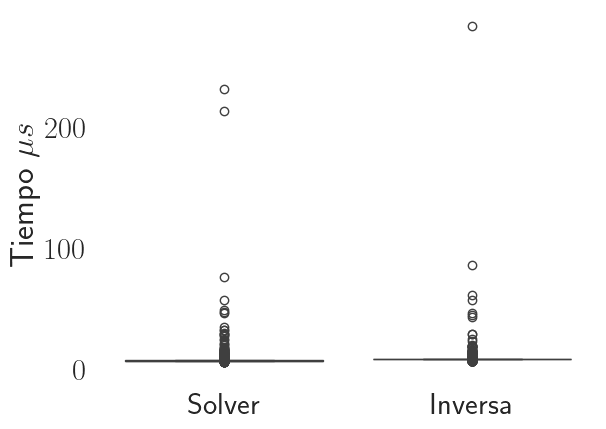
\includegraphics[width=0.5\textwidth]{../img/solver_inversa_gamma}
    \caption{Comparación de tiempos de cómputo entre Solver e Inversa}
    \label{fig:time_comparison}
\end{figure}

Los resultados se muestran en la Tabla~\ref{tab:solver_inversa_gamma}.

\begin{table}[H]
 \centering
\caption{Tiempo de ejecución de los métodos de solución}
\label{tab:solver_inversa_gamma}
\begin{tabular}{l|r|r}
 & Solver & Inversa \\ \hline
Media & 7.827 & 8.340 \\ \hline
Desviación estándar & 7.467 & 6.894 \\ \hline
Mínimo & 5.722 & 6.676 \\ \hline
Percentil 25 & 6.914 & 7.868 \\ \hline
Percentil 50 & 6.914 & 7.868 \\ \hline
Percentil 75 & 7.153 & 8.106 \\ \hline
Máximo & 230.789 & 283.241
\end{tabular}
\end{table}


De la Tabla~\ref{tab:solver_inversa_gamma}, se observa que el método de eliminación Gaussiana (Solver) es el más rápido en términos de tiempo de ejecución, en comparación con el método de inversa.
Este resultado es esperado, ya que el método de inversa requiere calcular la inversa de la matriz $I - \gamma P$, lo cual es computacionalmente costoso.

Por otro lado, se recomienda tener en cuenta este resultado al momento de seleccionar el método de solución a utilizar, ya que el tiempo de cómputo puede ser un factor importante en la elección del método.
Si bien el caso en particular no presenta diferencias significativas, en problemas más grandes, la diferencia en tiempo de cómputo puede ser considerable.

\line(1,0){\textwidth}
